%%%%%%%%%%%%%%%%%%%%%%%%%%%%%%%%%%%%%%%%%%%%%%%%%%%%%%%%%%%%%%%%%%%%%%%%%%%%%%%%
%%                           ONDER DE LOEP ARTIKEL                            %%
%%%%%%%%%%%%%%%%%%%%%%%%%%%%%%%%%%%%%%%%%%%%%%%%%%%%%%%%%%%%%%%%%%%%%%%%%%%%%%%%

\artikelfoto{Klaar voor de GRexit?}{}{Gerd Hautekiet  \\ Filip Moons \\Luc Van den Broeck}{img/grexit2.jpg}

\startcontents[inhoudloep]	% om inhoud voor het loep artikel te beginnen

\begin{multicols}{2}
	
	\inhoudstafelloep			% om inhoudstafel voor het loep artikel te tonen
	
	%% Gebruik \section{titel} en \subsection{titel} om genummerde tussentitels te maken
	\section{Inleiding}
In meer en meer scholen stapt men af van het grafisch rekentoestel en stapt men over op een laptop. Deze beweging is zeker versneld door het online lesgeven tijdens de corona-epidemie. De digisprong waarbij de minister veel geld vrijmaakt voor laptops, brengt dit allemaal nog in een hogere versnelling. Je kunt het niet maken om nog eens een behoorlijke som te vragen voor een grafische rekenmachine. En dus wordt de grafische rekenmachine naar de uitgang verwezen, de GR-exit dus. Veel wiskundeleerkrachten zijn hier niet zo blij mee. Dit komt nog eens bovenop de modernisering van het secundair onderwijs. Ze snakken naar rust...  Verandering is altijd moeilijk!

Het is niet de eerste keer dat we zo’n revolutie meemaken. Mijn vader had een rekenlat in zijn hemdzakje zitten. Ikzelf herinner me dit nog als leerling eind jaren '70 in het vijfde jaar. Ik had van mijn oudere broer een heuse rekenmachine overgekocht. Het was een groot zwaar en duur toestel, met rode cijfertjes, met een adapter en de batterij moest zowat dagelijks opgeladen worden. Mijn broer kocht voor zichzelf een ‘zwaarder’ model, eentje dat nog meer kon omdat hij naar de hogeschool ging. Ik was fier op mijn rekenmachine die veel minder kon dan een simpele rekenmachine die nu dikwijls in de eerste graad gebruikt wordt.

Ik herinner me vooral nog dat ik mijn rekenmachine niet in de wiskundeles mocht gebruiken want we zouden niet meer kunnen rekenen! Voor de oefeningen in de lessen fysica en chemie was er geen bezwaar dat ik die gebruikte. Ondertussen bleven we in de wiskundelessen tweedegraadsvergelijkingen oplossen met een discriminant die ofwel 0, negatief of een volkomen kwadraat was. Voor goniometrie en logaritmen hadden we altijd ons boekje met logaritmetafels bij. Maar meestal gingen de oefeningen over hoeken van 30°, 45° of 60° of de verwante hoeken. Wortelvrij maken van de noemer, integratiemethodes,  waren toen belangrijke vaardigheden waar heel wat onderwijstijd naar toe ging… Ik herinner me bij analyse ook nog het magische moment als je het domein, de snijpunten met de assen, de berekeningen van de asymptoten, de eerste en tweede afgeleide met hun tekenonderzoek samenbracht in een samenvattende tabel om dan een grafiek te kunnen tekenen van een nieuwe functie. De apotheose, alle puzzelstukjes vielen `in de plooi' of juist niet, maar dan kon je op zoek gaan naar een fout!


\end{multicols}
\afbeelding[11.5 cm]{img/UWgrexit}{}{}
\begin{multicols}{2}


Een tiental jaren later had ik voor het eerst een leerling die met haar zuur verdiende spaarcentjes een grafische rekenmachine gekocht had. Ook toen was het even zoeken: niet iedereen kon zich zo’n toestel permitteren, laat staan dat het een schoolstandpunt was om het te veralgemenen. Hier zijn toch ook een aantal jaren en veel vakvergaderingen overgegaan vooraleer er beslist werd dat iedereen vanaf het derde jaar zich een grafisch toestel moest aanschaffen. We moesten onze manier van lesgeven, oefeningen en toetsen aanpassen. En in het begin was dit ook zoeken. In plaats van een grafiek als resultaat van een oefening, werd de grafiek het vertrekpunt en stelden we daar vragen bij: bijvoorbeeld bereken de exacte positie van de buigpunten, kies een goed venster zodat de grafiek goed zichtbaar is of zoom in op een deel van de grafiek. We konden oefeningen geven die niet meer zo mooi uitkwamen. We konden vergelijkingen grafisch oplossen die algebraïsch niet op te lossen waren. We konden oplossingen die we algebraïsch berekenden direct verifiëren met de grafische rekenmachine.

De grafische rekenmachine heeft er zeker toe geleid dat ICT effectief gebruikt wordt in de wiskundelessen en wiskundeproefwerken, in tegenstelling tot eerdere pogingen waarbij er dan verhuisd moest worden naar een computerklas. De grafische rekenmachine is goed ingeburgerd in ons secundair wiskundeonderwijs. De handboeken hebben zich gaandeweg ook aangepast, mede door vele artikels in Uitwiskeling.

Ondertussen staan we dus opnieuw op zo’n keerpunt. Er zijn voor- en tegenstanders maar vooruitgang hou je niet tegen. Ik vind het helemaal niet erg dat ik geen vierkantswortels meer met de hand moet trekken, dat ik mijn logaritmetafels niet meer moet gebruiken... Dus laten we naar de toekomst kijken: het feit dat de digisprong ongeveer samenvalt met de modernisering van het secundair onderwijs, verplicht ons, leraren, om samen op zoek te gaan naar de mogelijkheden, de meerwaarde, de voordelen om met nieuwe technologische hulpmiddelen ons wiskundeonderwijs te overdenken.

En ja, er zijn ook praktische en didactische nadelen: de laptops nemen veel plaats in op de bank, ze zijn niet altijd opgeladen als je ze nodig hebt, er zijn niet genoeg stopcontacten in de klas of de leerlingen hebben geen lader bij, je ziet niet wat leerlingen op en achter hun scherm aan het doen zijn... 

Een klein rekentoestel kan handig zijn om praktische redenen. Hiermee kun je nog van alles doen: het simpele rekenwerk maar ook nog een aantal functies uit statistiek, tabellen, $3 \times 3$ matrices... Sommige leerkrachten zoeken nu naar oefeningen die beperkt blijven tot deze grenzen. Dit zien we niet graag: statistiek doe je toch veel beter met GeoGebra of Excel.

We kunnen ook op zoek gaan naar de mogelijkheden van de gsm, die de meeste leerlingen altijd bij hebben en die meestal wel opgeladen is! Die neemt geen plaats in, is handiger voor kort gebruik en er is een niet-storen-modus!

We willen zeker nog vermelden dat ook wij het niet allemaal weten. Deze loep is een eerste aanzet om over dit onderwerp na te denken. We zijn zelf ook zoekend en zijn daarom voor deze loep met verschillende mensen gaan praten die ondertussen al wat meer ervaring hebben maar ook nog steeds hun weg zoeken. De GRexit zal in de meeste scholen geleidelijk gebeuren, niet alle leerlingen zitten in hetzelfde traject: het kan bijvoorbeeld zijn dat de leerlingen van de eerste jaren enkel een laptop hebben maar dat de leerlingen van de hogere jaren nog wel een grafische rekenmachine hebben. Deze leerlingen zullen dit toestel uiteraard nog blijven gebruiken, maar voor sommige onderdelen van de leerstof is het gebruik van GeoGebra misschien toch ook al een meerwaarde.

Verder willen we benadrukken dat de technologie een hulpmiddel is, niet het doel van ons lesgeven. Leerlingen moeten generieke vaardigheden opdoen. Het gaat zeker niet uitsluitend om het bedienen van concrete tools. Bij de overgang van de grafische rekenmachine naar bijvoorbeeld \mbox{GeoGebra}, begin je ook niet van nul. De knoppen zijn anders, maar bijvoorbeeld het feit dat je het functieonderzoek start met de grafiek, dat je oplossingen van vergelijkingen numeriek bepaalt... dat verandert niet. 

Stof genoeg om vooruit te kijken: welke meerwaarde biedt de laptop ten opzichte van de grafische rekenmachine?

In paragraaf 2 gaan we verder in op GeoGebra dat zowat het nieuwe standaardpakket lijkt te worden, en in paragraaf 3 kijken we hoe het nu moet met toetsen en examens. In paragraaf 4 geven we enkele voorbeelden uit de klas waarbij we de meerwaarde van het gebruik van de laptop willen benadrukken of waarbij we proberen met nieuwe ogen te kijken naar oudere onderwerpen. In de volgende paragraaf leggen we uit welke rol Python kan spelen bij de GRexit. In paragraaf 6 schetsen we een theoretisch kader om kritisch naar de rol van ICT in het wiskundeonderwijs te kijken. In de laatste paragraaf kijken we even naar de situatie in het hoger onderwijs en kijken we even over het muurtje in Nederland.

	\section{GeoGebra}
GeoGebra heeft ondertussen zijn plaatsje gevonden in de meeste scholen. Het is gratis, vlot toegankelijk en bruikbaar voor heel veel topics van het wiskundeonderwijs. Leerlingen kunnen de mogelijkheden van het programma gaandeweg leren kennen van het eerste tot het zesde jaar, wanneer het nut heeft en een meerwaarde geeft voor een bepaald leerplanonderdeel.

Het gebruik van GeoGebra kan op verschillende manieren: ofwel vertrek je van een leeg tekenblad en bouw je bewust bepaalde constructies of functies zelf op, ofwel maak je dankbaar gebruik van het vele materiaal dat iemand anders al voor je gemaakt heeft. Wellicht is de combinatie van de twee werkwijzen het meest zinvolle.

Veel leerlingen in het eerste jaar kunnen met een beknopte handleiding de verschillende knoppen in het programma zelfstandig leren gebruiken. De leerkracht kan zich dan meer focussen op de leerlingen die hulp nodig hebben. Hieronder in \autoref{geogebrameetkunde} zie je een voorbeeld om stapsgewijs de basisconstructies van meetkunde te laten ontdekken.



\end {multicols}

\afbeelding [15,4cm] {img/Lmeetkunde_en_ICT.JPG}{Meetkunde en ICT met GeoGebra}{geogebrameetkunde}

\begin{multicols}{2}

De bedoeling van het gebruik van GeoGebra is om meetkunde te leren, functies te leren onderzoeken, statistiek te doen en te begrijpen. GeoGebra is niet het doel maar een middel. 
Bij meetkunde kun je nagaan of een figuur goed gemaakt is. Heeft de leerling de constructie goed uitgevoerd? Daarvoor moet je niet alle stappen in de constructie nakijken maar door aan bepaalde punten te trekken, merk je of de constructie goed gebeurd is. In \autoref{rechthoek} is en blijft de linkse vierhoek een rechthoek, eender welk hoekpunt je verplaatst. De rechtse vierhoek is geen rechthoek en dat merk je zeker als je één van de hoekpunten probeert te verplaatsen.

\afbeelding {img/Lrechthoek.png}{Twee rechthoeken?}{rechthoek}

GeoGebra kun je ook gebruiken op de smartphone: dit kan  handig en praktisch zijn voor een gewone les. Bijvoorbeeld als leerlingen een tekentabel bij een functie gemaakt hebben en ze hun antwoord snel willen controleren met een grafiek. De smartphone neemt niet veel plaats in op de bank, leerlingen hebben dit toestel meestal bij en die batterij is meestal niet plat! 
Een nadeel is dat leerlingen nog veel andere dingen kunnen doen met hun smartphone. Hetzelfde geldt uiteraard ook voor laptops. Ook via die apparaten kunnen de leerlingen video’s kijken en sociale media volgen. Gericht gebruik van smartphones en laptops, aandacht voor digitale geletterdheid, impulsgedrag leren controleren, zijn dingen die ook aangeleerd moeten worden op school. Met gericht gebruik (alleen als de leraar de opdracht of toestemming gegeven heeft voor gebruik) hebben leerlingen toch voldoende rust en plukken ze de voordelen van technologische ontwikkelingen en worden ze tegelijkertijd goed voorbereid op de digitale samenleving. Afspraken op schoolniveau werken het beste: als alle leraren dezelfde regels hanteren, staan ze ook sterker bij eventuele conflicten over smartphones in de klas.

	\section{Wat met examens en toetsen?}
Ik ben bij de grafische rekenmachine nooit voorstander geweest van geheugens wissen… Als leerlingen bepaalde formules in het geheugen van hun rekenmachine konden stoppen en dus hun machine konden programmeren, was dit meestal iets dat ze op eigen initiatief hadden bijgeleerd. Dit valt alleen maar toe te juichen. Als deze formules en dergelijke ook konden doorgegeven worden via een fysieke verbinding tussen twee rekenmachines, veranderde de zaak, maar ook hier gold meestal: als leerlingen niet wisten wat deze formules betekenden, konden ze ze ook niet gericht inzetten in de les of bij een toets.

Een concreet voorbeeld: in het vijfde jaar hadden de meeste leerlingen een programmaatje 'vkv' of 'vierkantsvergelijking' in hun grafische rekenmachine zitten om de discriminant en de oplossingen van een tweedegraadsvergelijking te berekenen. Het voordeel was dat ik bij oefeningen over veeltermfuncties veel oefeningen kon maken zonder elke keer te moeten wachten tot iedereen de juiste waarde voor de discriminant gevonden had. Moesten de leerlingen deze formule dan niet meer kennen? Toch wel, dit loste ik op door er oefeningen tussen te steken met een parameter zodat ze de formule toch nodig hadden. Het programma vkv heeft me dus veel tijdwinst opgeleverd! En als leerlingen dit tijdens de lessen altijd mogen gebruiken, zie ik niet in waarom ze dat niet zouden mogen gebruiken bij een toets of examen. 

En ja, het is ooit gebeurd dat leerlingen er in geslaagd zijn om een hele cursus met veel tekst in hun rekenmachine te steken. Dan krijg je natuurlijk een ander verhaal. Dit staat gelijk met spieken. Meestal zie je dan aan het verdachte gedrag van een leerling dat hij of zij vooral aan het scrollen is en dat is niet het normale gebruik van een rekenmachine! Goed actief toezicht doen is en blijft hier nog altijd essentieel. 

Bij een computer kun je natuurlijk nog veel verder gaan, leerlingen zouden ook onderling antwoorden en bestanden met elkaar kunnen uitwisselen. 

Het is dus niet allemaal vooruitgang! De laptop gebruiken op een examen levert meer rompslomp op dan de grafische rekenmachine. We zien de proefwerken evolueren naar een deel zonder laptop, al of niet met een eenvoudig rekentoestel, en een ander deel met de laptop. Daarom gaan we iets dieper in op de examenmodus van GeoGebra.  

\end{multicols}
\afbeelding[11,5 cm]{img/UWdwangbuis}{}{}
\begin{multicols}{2}

\subsection*     {Examenmodus van GeoGebra}
Er bestaan verschillende versies van GeoGebra. Om de examenmodus te kunnen gebruiken moet je kiezen voor de offline grafische rekenmachine. De online rekenmachine kun je niet in examenmodus zetten. Kies dus voor de GeoGebra Classic 6 of de GeoGebra Suite App. Deze programma's ondergaan voortdurend updates. Je moet dus zelf regelmatig op zoek gaan naar recente info en tutorials blijven nuttig.

Om in de examenmodus te gaan, klik je op de menubalk en kies je voor de Examenmodus (\autoref{opstarten}).

\afbeelding [6 cm]{img/Lexamenmodus1.png}{Opstarten examenmodus}{opstarten}

Er verschijnt een dialoogvenster (\autoref{mogelijkheden}) waarin je kunt kiezen om alle gebruiksmogelijkheden te gebruiken of om het CAS en/of 3D tekenvenster te deactiveren.

\afbeelding [6 cm]{img/Lexamenmodus2.png}{Alle of sommige mogelijkheden}{mogelijkheden}
Klik op \emph{Start het examen}. De Examenmodus start dan: GeoGebra gebruikt heel het scherm, je krijgt geen andere taakbalken meer te zien. In de balk bovenaan zie je dat de examenklok gestart is en welke onderdelen eventueel geblokkeerd zijn. 

De Examenmodus sluit je af door in het menu (de drie streepjes rechts bovenaan) \emph{Bestand/Examenmodus afsluiten} te kiezen.
Je bevestigt door op \emph{Afsluiten} te klikken (\autoref{afsluiten}, \autoref{bevestigen}).
\afbeelding [5 cm]{img/Lexamenmodus3.png}{Afsluiten Examenmodus}{afsluiten}
\afbeelding [6 cm]{img/Lexamenmodus4.png}{Afsluiting bevestigen}{bevestigen}

Vervolgens verschijnt er automatisch een Examen Logboek. Dit moet je door je leerlingen laten opslaan en kun je dan eventueel via smartschool laten uploaden op het einde van het examen, net voor het verlaten van het lokaal bijvoorbeeld. 
\afbeelding [5.5 cm]{img/Lexamenmodus5.png}{Logboek}{}
Als een leerling geprobeerd heeft iets anders te doen op zijn laptop, wordt de bovenste balk rood gekleurd en verschijnt dit ook in het logboek.
Heel af en toe kan GeoGebra vastlopen als een leerling erg knoeit met invoeren. Je kunt dan geforceerd stoppen (met Ctrl Alt Delete). Je moet wel een nieuwe examenmodus opstarten. Schrijf als toezichthouder onregelmatigheden op. 

Enkele tips:

Zorg dat je de Examenmodus eerst eens test met de leerlingen bij een gewone toets in de klas vooraleer je dit toepast op een examen. Benadruk dat de leerlingen altijd de leraar moet verwittigen als er iets abnormaals gebeurt op zijn of haar computer. Laat de leerlingen allemaal op hetzelfde moment in Examenmodus gaan en deel daarna pas de vragen uit. Zorg dat je als leraar de schermen ziet. Ofwel laat je alle leerlingen aan de andere kant van de bank zitten ofwel, veel eenvoudiger, ga je zelf aan de andere kant van de klas staan! Ook leerlingen kunnen elkaars schermen zien, veel meer dan elkaars papieren. Een tablet of een iPad kun je horizontaal leggen, maar bij een gewone laptop is die mogelijkheid er niet.



	\section{Voorbeelden uit de klas}
	Het blijft uiteraard belangrijk dat je leerlingen toch nog algebraïsche vaardigheden laat inoefenen en dat je bepaalde zaken met en andere zonder computer laat doen. Je kunt nog altijd oefeningen laten maken zonder computer maar het mooie is juist dat je algebraïsche berekeningen kunt ondersteunen door grafisch te vergelijken. Je kunt dankzij het computerrekenwerk meer probleemoplossing doen: vertaal het probleem naar een wiskundig probleem, los dit op met de computer en vertaal de oplossing terug naar je probleem. 
	Het is een belangrijke taak voor de leraar zich af te vragen hoe je oefeningen kunt aanpassen zodat ze toch zinvol zijn.
	
		We geven hieronder enkele voorbeelden waarbij ICT echt een meerwaarde is of waar we oefeningen aangepast hebben aan de nieuwe technologie. 
	
	\subsection{Kenmerken van parabolen }
Bij de studie van kwadratische functies leren de leerlingen de symmetrie-as en de top bepalen, de snijpunten met de assen... Bij het oplossen van problemen over dit onderwerp, kunnen leerlingen gebruik maken van GeoGebra. Ook als ze de software gebruiken, moeten ze nog heel goed weten wat ze moeten doen.


Uit DELTA-T 4A werkboek, Wolters-Plantyn: Johan is een echte tuinliefhebber. Op een zonnige dag besproeit hij zijn planten en bloemen, zoals afgebeeld op de figuur.

\afbeelding [8cm] {img/Ljohan.jpg}{Een waterstraal in de vorm van een parabool}{}

	\begin{itemize}
	\item Bepaal het voorschrift van de functie waarvan de waterstraal de grafiek vormt. Teken de grafiek van deze functie.
	\item Op welke hoogte houdt Johan de tuinslang vast?
	\item Hoe hoog moet Johan de tuinslang houden om de planten die 1m verder staan te kunnen besproeien?
	\item Hoe ver moet Johan vooruit stappen om de planten die 1m verder staan te kunnen besproeien vanop 1m hoogte?
	\end{itemize}
\afbeelding [8cm] {img/Lparabool.JPG}{De waterstraal in GeoGebra}{}


\subsection{Telecomoorlog in Gent}





Het voorbeeld in \autoref{overgangsmatrices} (uit \url{www.geogebra.org/m/ysdsbbrx}) gaat over overgangsmatrices. We gaan er van uit dat je in de klas het begrip overgangsmatrix al behandeld hebt, dat de leerlingen al zelf zo'n matrix opgesteld hebben en dat ze weten hoe ze er mee moeten rekenen.  

In Gent woedt een ware telecomoorlog tussen Base 10, Proxiplus en Reëlenet. Gebruik de applet om het effect van verschillende parameters te onderzoeken:
\begin{itemize}
\item Reken de situatie uit na verschillende tijdstippen.
\item Laat zien dat de verdeling stabiliseert op de grafiek en bij de berekeningen. 
\item Laat zien dat de begintoestand geen invloed heeft op de evenwichtssituatie door verschillende beginverdelingen te proberen (met hetzelfde totaal) en de evolutie te tonen via het traject.
\end{itemize}

\end{multicols}
\afbeelding {img/Ltelecomoorlog.jpg}{Overgangsmatrices en de telecomoorlog}{overgangsmatrices}
 
\begin{multicols}{2}

\begin{itemize}
\item Pruts met de overgangswaarschijnlijkheden en bekijk het effect op de evenwichtssituatie (bijvoorbeeld Proxiplus doet een prijsverlaging en overhaalt maandelijks 10\% extra klanten van Reëlenet om over te stappen).
\end{itemize} 

 De meerwaarde van dergelijke toepassingen is dat je voorbereide applets kunt gebruiken. De leerlingen kunnen snel en efficiënt onderzoekend bezig zijn. Het mag natuurlijk niet blijven bij wat knopjes verslepen, de oefening moet gevolgd worden door een analyse van de resultaten.

\subsection{Families krommen}
Bij het onderzoek van families functies gebruiken we dikwijls één of meer parameters. Met behulp van GeoGebra kunnen we veel gemakkelijker de rol van de parameter(s) duidelijk maken.  Ik denk bijvoorbeeld aan de parabolen $y=a \cdot x^2$, de algemene sinusfunctie $y=a \sin (b(x-c))+d$, de exponentiële functie $y=a^x$.
	
Voer in GeoGebra de functie in met een parameter en er verschijnt vanzelf een schuifbalk. Je kunt de waarden van de parameter simpelweg veranderen door het bolletje over de schuifbalk te verslepen of je kunt automatisch de waarden laten veranderen door op het pijltje te klikken. Ook het bereik en de stapgrootte van de parameter kun je gemakkelijk veranderen.
\afbeelding {img/Lparabolen_parameter}{Parabolen met een parameter}{}
Mogelijke vragen voor de studie van de parabolen:
\begin{itemize}
	\item Bij elke waarde van de parameter hoort er precies één functie: teken de grafiek van de functie voor $a=-2, a=-1, a=0, a=1, a=2, a=1,5$.
	\item	Welk verband merk je tussen de waarde van $a$ en de ligging van de grafiek?
	\item Hoe kun je de waarde van $a$ terugvinden op de grafiek?
	\item	Welke waarde moet de parameter hebben om door het punt $(2,\;5)$ te gaan?
	\item Alle parabolen van de vorm $y=a \cdot x^2$ gaan door eenzelfde punt, welk?
	\item	Welke waarden mag de parameter $a$ (niet) aannemen?
	\end{itemize}

Je kunt het commando Rij$(ax^2, a,1,5,2)$ gebruiken om voor elke waarde van de parameter $a$ vanaf de beginwaarde tot en met de eindwaarde en met een zelf gekozen stapgrootte de grafieken samen op het scherm te tekenen. 
	
\afbeelding {img/Lrij_parabolen.JPG}{Een rij parabolen}{}		
	
\subsection{Extremumproblemen}

Met de app van \autoref{extremum} (met dank aan Mathias Stichelbaut, zie \url{www.geogebra.org/m/ksbx9bw6}) kun je een concreet extremumprobleem visualiseren: een vierkant en en een cirkel hebben samen een omtrek van 100 m. Voor welke afmetingen is de totale oppervlakte minimaal? 

Je kunt heel gemakkelijk laten zien wat het effect is van het veranderen van de gekozen onafhankelijke veranderlijke. Vervolgens kun je het probleem op de klassieke manier laten berekenen en tenslotte je gevonden oplossing verifiëren.  

\end{multicols}
\afbeelding [13,5 cm]{img/Lextremumproblemen.jpg}{Visualisatie van een extremumprobleem}{extremum}	
	
\begin{multicols}{2}

	
	\subsection{Convergentie van een rij met \mbox{GeoGebra}}
	We laten zien hoe je GeoGebra kunt gebruiken bij het aanbrengen van de $\varepsilon$-$N$-definitie van limiet van een rij. We beperken ons tot het geval waarbij de rij convergeert (met andere woorden waarbij die een getal als limiet heeft). Het geval waarbij de rij divergeert naar plus of min oneindig kan op een analoge manier met GeoGebra ondersteund worden.
	
	Als we de grafiek van de rij $u_n=\frac{6n+4\cdot (-1)^n}{n}$ bekijken, zien we dat de termen ‘naar 6 gaan’ als we verdergaan in de rij (\autoref{rij1}). De rij ‘convergeert’ naar 6. Of nog: $\lim_{n \rightarrow \infty}{u_n}=6$. Als je in GeoGebra horizontaal uitzoomt, lijken de grafiekpunten meer en meer op de rechte $y=6$ te liggen. Voor veel leerlingen, ook in wiskundeklassen, volstaat de formulering met ‘gaan naar’. Je kunt iets preciezer zijn door te zeggen: $u_n$ komt ‘willekeurig dicht’ bij 6 (zo dicht bij 6 als je wilt) als je het rangnummer ‘groot genoeg’ neemt.
	
	
Maar wat betekent dat precies? Hoe dicht wil je dat $u_n$ bij $y=6$ komt? Hoe groot is ‘groot genoeg’?
\end{multicols}
\afbeelding [11 cm] {img/Lrij1.png}{De rij convergeert naar 6.}{rij1}	
	
\begin{multicols}{2}

Voor sterkere of kritischere leerlingen kun je hier met de $\varepsilon$-$N$-definitie een antwoord op geven:

$\lim_{n \rightarrow \infty}{u_n}=6$

betekent:

$\forall \varepsilon >0:\exists N: n>N \Rightarrow 6-\varepsilon<u_n<6+\varepsilon$

Of nog: voor elke strook met breedte $2\varepsilon$ rond $y=6$, hoe smal ook, als je in de rij verder gaat dan een bepaald rangnummer $N$, dan liggen de grafiekpunten in die strook. Merk op dat je het rangnummer $N$ mag aanpassen aan $\varepsilon$. Neem je een kleinere $\varepsilon$ (en dus een smallere strook), dan moet je $N$ groter nemen.

Dit wordt goed geïllustreerd met schuifknoppen in GeoGebra. De ene leerling mag de $\varepsilon$-knop bedienen en de andere leerling moet de $N$-knop aanpassen, zodat alle punten rechts van $x=N$ binnen de strook liggen (\autoref{rij2}: we hebben verticaal een beetje ingezoomd).

Je ziet niet altijd goed of een grafiekpunt binnen of buiten de strook ligt. Dit motiveert het algebraïsch berekenen van $N$ aangepast aan een willekeurige $\varepsilon$. Dit werken met ongelijkheden is typisch voor de analyse zoals die in een universitaire cursus wordt bedreven. In dit geval is het nog eenvoudig: de lezer kan met ongelijkheden verifiëren dat je hier voor $N$ een natuurlijk getal moet nemen dat groter is dan of gelijk aan $\frac{4}{\varepsilon}$. Voor $\varepsilon=0,14$ geeft dit $N \geq 29$. De leerling met de $N$-knop bij \autoref{rij2} deed het goed. Een kleinere $N$ mocht hij niet nemen; hij had wel gerust een grotere $N$ mogen nemen. Het is niet nodig om de kleinst mogelijke $N$ te zoeken.
\end{multicols}
\afbeelding [11 cm]{img/Lrij2.png}{De $\varepsilon$-$N$-definitie met GeoGebra}{rij2}	
	
\begin{multicols}{2}

Enkele technische details: de rijen die je in \mbox{GeoGebra} maakt, zijn eigenlijk altijd eindig. We maakten een rij met 100 termen: u = \mbox{Rij((6n+4(-1)\^{}n)/n,n,1,100)}. GeoGebra tekent de rij niet vanzelf, je moet er eerst een rij punten mee maken:
grafieku=Rij((n,u(n)),n,1,100). 

Je vindt online gelijkaardige GeoGebrafiguren die een beetje gesofisticeerder zijn. Bv. \url{www.geogebra.org/classic/D7GBC0x9}: de punten binnen de strook worden automatisch groen gekleurd en de punten erbuiten rood. 


\subsection{De normaalverdeling met GeoGebra}
Je kunt GeoGebra makkelijk gebruiken om oefeningen op te lossen over de normaalverdeling. Dit kon je uiteraard ook met de grafische rekenmachine. Voor leerlingen die vroeger geen grafische rekenmachine hadden, kun je verder gaan dan de 68-95-99,7-regel. Je kunt genoeg variatie in de oefeningen steken om te zien welke leerlingen de leerstof begrepen hebben en welke niet.  

Een drankfabrikant onderzoekt de inhoud van 250ml-flesjes op één van zijn lijnen. De inhoud van de flesjes is normaal verdeeld met $\mu= 249,3$ ml en $\sigma = 2,777$ ml.
\begin{itemize}
\item Bereken het percentage flesjes met een inhoud kleiner dan 252 ml. 
\item Bereken het percentage flesje met een inhoud groter dan of gelijk aan 249 ml. 
\item Hoeveel percent van de flesjes heeft een inhoud tussen 251 ml en 255 ml?
\item  Bereken onder welke inhoud de 10\% minst gevulde flesjes zich bevinden.
\item Bereken tussen welke inhouden de 50\% middelste flesjes zich bevinden. 
\end{itemize}
\afbeelding {img/Lflesjes.jpg}{Percentage flesjes met een inhoud lager dan 252 ml}{} 


	\section{Python}
Met de exit van de grafische rekenmachine neemt het gebruik van wiskundige apps op de computer of de smartphone toe. Echter, het is niet altijd zo eenvoudig om een app te vinden die precies doet wat je in gedachten hebt. Zo vind je bijvoorbeeld geen programma om een kansexperiment met munten of dobbelstenen te simuleren dat net iets teveel afwijkt van het gewone tossen of het werpen met kubusvormige dobbelstenen. In zulke gevallen is het handig zelf te kunnen programmeren. 
	
	De leerplannen in de tweede graad van de doorstroomfinaliteit ondersteunen deze computervaardigheid met het item \emph{computationeel denken}. Ze formuleren het als volgt:
	
	\begin{citaat}
		De leerlingen ontwerpen algoritmes om problemen digitaal op te lossen.
	\end{citaat}
	
	Naast het ontwikkelen van algoritmes wordt er aandacht besteed aan structuurelementen in een computerprogramma zoals: de opeenvolging, de begrensde herhaling, de voorwaardelijke herhaling, de keuzestructuur ... Verder komen er nog de grammaticale spelregels van een programmeertaal (de \emph{syntactische regels}) in de leerplannen aan bod: de datatypes, de operatoren, de functiedefinities, ... De leerplandoelstellingen van het computationele denken zijn erg amibitieus geformuleerd. 
	
	Los van de discussie of deze doelstellingen niet beter verwezenlijkt worden in een apart vak informatica, geven we in deze paragraaf tips hoe we aan de verwachtingen kunnen voldoen binnen een beperkt tijdsvenster. In de discussie of we ook niet kunnen leren programmeren op een grafische zakrekenmachine nemen we wel een standpunt in. Op het minischermpje van een grafische zakrekenmachine kun je onmogelijk het overzicht van een programma bewaren tenzij het zeer kort en elementair is.
	
	Volgens de leerplannen kan een school ervoor kiezen om de bovenvermelde doelstelling te realiseren voor een geschikte actuele programmeeromgeving, die aansluit bij de studierichting en het te verwachten vervolgtraject. Python is zo'n actuele programmeertaal. Sinds 2019 is ze wereldwijd de meest gebruikte programmeertaal (zie Most popular programming languages from 1965 to 2020). Python is in het begin van de jaren '90 ontwikkeld door de Nederlander Guido Van Rossum. De programmeertaal heeft een groot bereik aan toepassingsmogelijkheden. Hoewel, voor gespecialiseerde doeleinden zoals gaming, webdevelopment, data-analyse, ... gebruik je beter meer gespecialiseerde software.
    
    Python heeft het voordeel van een overzichtelijke programmastructuur zonder wildgroei aan haakjes. De \emph{indentations} of inspringingen zorgen ervoor dat de hiërarchie tussen de programmablokken meteen in het oog springt. 
    
    Een ander pluspunt van Python is de \emph{ducktyping}. Dit wil bijvoorbeeld zeggen dat een variabele die de schijn wekt een geheel getal te zijn, als een geheel getal geïnterpreteerd zal worden. Een variabele die de schijn wekt een reëel getal te zijn, zal als een reëel getal geïnterpreteerd worden. Python voelt meestal intuïtief aan om welk soort variabele het gaat zonder dat het type op voorhand gedeclareerd hoeft te worden. De term \emph{ducktyping} komt van een Engelse zegswijze: \emph{If it looks like a duck, swims like a duck, and quacks like a duck, then it probably is a duck}.
    
     \afbeelding [3cm] {img/pythonlogo.png}{Het logo van Python: een gele en een blauwe slang. It looks like a duck.}{fig:slang}
	
	Werken met \emph{packages} is ook een belangrijk pluspunt van Python. Door bepaalde packages bij  het begin van een programma te laden, worden er nieuwe functionaliteiten aan Python toegevoegd. Zo gebruiken we het pakket
	\begin{itemize}
	\item \emph{Numpy} voor het numeriek berekenen van functiewaarden, 
	\item \emph{Matplotlib} voor het tekenen van grafieken, 
	\item \emph{Sympy} voor symbolisch rekenwerk, 
	\item \emph{Pandas} voor statistische berekeneningen;
	\item \emph{Random} voor het rekenen met kansvariabelen. 
	\end{itemize}
	Dit zijn enkele van de bekendste bibliotheekprogramma's van Python.
	
	Om deze en nog vele andere redenen is Python een populaire keuze als programmeertaal voor leerlingen van het secundair onderwijs. 
	
	Een attitude die onze programmerende leerlingen moeten aanleren is het werken in een dubbel scherm: eentje om te programmeren en eentje om opzoekingswerk te verrichten. Een programmeertaal leren is een beetje zoals een taalbad nemen. Je wacht niet tot je voldoende grammaticale regeltjes geleerd hebt maar je begint meteen te spreken of te schrijven. Pas als de tegenpartij (Python dus) je niet begrijpt, start je met opzoekwerk.
	
	\subsection{Starten met Python}
	
	Er zijn verschillende manieren om in Python te werken: online of offline, in een community of alleen, met automatische syntaxcontrole of zonder, enz.
	
	Het afgelopen jaar zijn er in Vlaanderen nascholingen geweest over het programmeren in Python via het platform \emph{Dodona} ontwikkeld aan de UGent. Op het internet worden er programmeeromgevingen aangeraden zoals \emph{Visual Studio Code}. Hoewel deze omgevingen waardevol zijn, gaan we er in deze loep niet verder op in. We stellen twee minder geavanceerde manieren en directere werkwijzen voor: programmeren in de opdrachtregel en programmeren via Replit.
	
	\subsubsection*{Programmeren in de opdrachtregel}
	De zuiverste manier om Python te gebruiken is via de \emph{opdrachtregel}. Toegegeven, je werkt dan in een minimalistische en oubollige omgeving met een zwarte achtergrond die erg doet denken aan de programma's uit de vroege jaren '90. 
	
	Voor je kunt beginnen, moet je Python \mbox{downloaden}. Kies hierbij voor versie 3.9 of versie 3.10. Tegen de tijd dat deze loep verschijnt is er waarschijnlijk ook al een volwaardige versie 3.11 ter beschikking. Na het downloaden van Python start je een interactieve Pythonsessie door in de opdrachtregel in Windows \emph{Python} of \emph{Python3} in te geven en op \emph{enter} te drukken. De windowsprompt verandert nu in het $>>>$-teken, zie \autoref{fig:opdrachtregel}. 
	
	De nieuwe prompt geeft aan dat je een Python-programmacode mag beginnen te typen. In \autoref{fig:opdrachtregel2} zie je hoe je met eenvoudige en heldere instructies $2^{10}$ kunt berekenen, hoe je een tekst op het scherm kunt laten verschijnen en hoe je vijf opeenvolgende kwadraten op het scherm kunt afdrukken.
	
	Nadeel van deze werkwijze is dat ze weinig ruimte laat voor correcties in programma's. Tik je een foutje in een instructie, dan moet je programmalijnen helemaal opnieuw ingeven. Werken vanaf de opdrachtregel is bijgevolg eerder geschikt om snel te controleren of een bepaalde instructie door Python aanvaard wordt.
	
	\end{multicols}
		\afbeelding {img/opdrachtlijn.jpg}{Python via de opdrachtregel}{fig:opdrachtregel}
		\afbeelding [10cm]{img/opdrachtlijn2.jpg}{Enkele programmalijnen in Python via de opdrachtregel}{fig:opdrachtregel2}
	\begin{multicols}{2}
	
	Misschien valt het je nu al op dat notaties in Python kunnen afwijken van wat we gewoon zijn in de wiskunde en op de grafische rekenmachine. Een machtsverheffing noteren we met een dubbele asterisk. En met \emph{range(5)} bedoelen we niet de gehele getallen van 1 tot en met 5 maar wel van 0 tot en met 4. Deze onverwachte notaties vormen echter maar een klein drempeltje. Leerlingen zijn het snel gewoon.

	\subsubsection*{Replit}
	
	Wie niet houdt van het installeren van programma's op de eigen computer, vindt waarschijnlijk zijn gading in het online programma \emph{Replit}, vroeger gekend als \emph{Repl.it}. Replit werd in 2016 ontwikkeld met als doel om in teamverband te kunnen samenwerken aan het schrijven van programmacode en het kunnen ontwikkelen van apps en websites. Het hoofdkwartier van Replit ligt in San Francisco, California. Replit ondersteunt een vijftigtal talen waaronder Python, Java, C++ en HTML. Repl is een acroniem voor Read-Evaluate-Print-Loop. 
	
	Op het internet vind je tal van online omgevingen om Python-code in te voeren. De meeste omgevingen zijn erg basic. Je kunt vaak geen packages importeren in deze online omgevingen en dat is een zware beperking. Replit ondersteunt deze packages wel. Een zwakker punt van Replit is de foutenanalyse. Wanneer een lopend programma onderbroken wordt door een fout, geeft Replit duidelijk aan waar de fout zit, maar vaak wordt er niet veel uitleg bij gegeven. 
	
	\afbeelding [3cm]{img/replitlogo.jpg}{Het logo van Replit}{fig:replit}
	
	Wij vinden Replit een ideale omgeving voor leerlingen van de tweede graad die korte programma's willen schrijven en die hierbij niet teveel digitale rompslomp willen overwinnen. Programma's die gemaakt zijn in Replit, kunnen eenvoudig in de cloud bewaard worden. Je kunt aanvinken of de community deze programma's mag zien en recycleren. En tot slot, net als alle andere omgevingen die we hier voorstellen, is het basispakket van Replit gratis, met inbegrip van onder andere 500MB schrijfruimte en het aanmaken van samenwerkingsgroepen tot en met 10 gebruikers.
	

	\subsection{Toepassingen voor het derde jaar}
	
	Hoewel de verleiding bestaat om tamelijk ver te gaan in het programmeren, raden wij aan om het in de tweede graad sober te houden. Programma's schrijven kan aanvankelijk vervangen worden door programma's verklaren of programma's aanvullen. Ook raden we aan om de eerste programma's kort te houden en de structuurelementen (keuze, begrensde herhaling, voorwaardelijke herhaling ...) niet teveel te mengen. 
	
	De programmeeropdrachten kunnen best ontleend worden aan de leerstof die op dat moment aan bod komt in de les. In het derde jaar zou dit een opdracht over vierkantswortels kunnen zijn of over de stelling van Pythagoras. In het vierde jaar zijn er mogelijkheden met het oplossen van willekeurige driehoeken of het maken van moeilijkere berekeningen rond parabolen. Het voorstel uit de leerplannen over het programmeren van de algoritmes van Prim, Kruskal en Dijkstra echter lijken ons nauwelijks haalbaar in de tweede graad.
	
	Belangrijk is wel dat de leerlingen beseffen dat computerprogramma's problemen aankunnen die te lastig zijn voor een grafische rekenmachine. In deze loep geven we enkele voorbeelden waarbij dit duidelijk wordt.
	
	\end{multicols}
	
	\begin{lesactiviteit}{Pythagoreïsche viertallen}
	
	In de vorige les heb je berekend dat de ruimtediagonaal $r$ van een balk met ribben $a$, $b$ en $c$ gelijk is aan $\sqrt{a^2+b^2+c^2}$. Dit kon je aantonen door de stelling van Pythagoras toe te passen in twee verschillende rechthoekige driehoeken, die in de balk terug te vinden zijn.
	
    \afbeelding[8 cm]{img/pythagorasbalk.jpg}{}{}
	
	\begin{vraagenantwoord}
		\vraag{Zoek gedurende vijf minuten naar zoveel mogelijk gehele ribben $a$, $b$ en $c$ die zorgen voor een gehele ruimtediagonaal van een balk.}
		\antwoord{Het kost een beetje speurwerk. Een van de kleinste voorbeelden is $a=1$, $b=2$ en $c=2$. Je kunt narekenen dat $r=3$ in dit voorbeeld. Een ander voorbeeld is $a=2$, $b=3$ en $c=6$, waarbij $r=7$.}
	\end{vraagenantwoord}
	
	Viertallen $(a, b, c, r)$ van natuurlijke getallen die van nul verschillen en waarvoor $a^2+b^2+c^2=r^2$, noemen we Pythagoreïsche viertallen. Er bestaan oneindig veel Pythagoreïsche viertallen.
	
	\begin{vraagenantwoord}[resume]
		\vraag{Zoek gedurende vijf minuten naar zoveel mogelijk Pythagoreïsche viertallen $(a, b, c, r)$ met getallen $a$, $b$ en $c$ strikt kleiner dan 20. Denk je dat je ze allemaal gevonden hebt?}
		\antwoord{Zonder computerprogramma is het onbegonnen werk om ze allemaal te vinden.}
	\end{vraagenantwoord}
	
	Hieronder geven we een (onvolledig) Pythonprogramma waarmee je deze viertallen kunt berekenen. De rode programmalijnen moet je zelf nog aanvullen. Over dit programma stellen we je verderop nog enkele vragen.\\
	
	
	\begin{kader}{Python}{Berekening van Pythagoreïsche viertallen}
    1. \qquad  import math\\
    2. \\
    3. \qquad def viertallen(n):\\
    4. \qquad \qquad for c in range(1,n):\\
    5. \qquad \qquad \qquad for b in range(1,c+1):\\
    6. \qquad \qquad \qquad \qquad for a in range(1,b+1):\\
    7. \qquad \qquad \qquad \qquad \qquad \textcolor{red} {r= ..........}\\
    8. \qquad \qquad \qquad \qquad \qquad \textcolor{red} {if ............ \quad :}\\
    9. \qquad \qquad \qquad \qquad \qquad \qquad print(a, b, c, int(r))\\
    10. \\
    11. \quad \, viertallen(20)\\
    \end{kader}
    

    In regel 1 importeren we het bibliotheekprogramma \emph{math} waarmee we onder andere  vierkantswortels kunnen berekenen. Zo komen we er bijvoorbeeld achter dat math.sqrt(25) gelijk is aan 5.
    
    Alle Pythagoreïsche viertallen waarbij $a$, $b$ en $c$ kleiner zijn dan $n$ worden berekend in het programmablok van lijn 4 tot en met lijn 9. In de bovenstaande opgave was $n=20$. Merk op dat het hele programmablok een tab (of vier spaties) naar rechts inspringt.
    
    Voor alle waarden $c$ van 1 tot en met $n-1$ wordt het programmablok van lijn 5 tot en met lijn 9 achtereenvolgens doorlopen. In de bovenstaande opgave gaat $c$ van 1 tot en met 19. Voor alle waarden $b$ van 1 tot en met $c$ wordt het programmablok van lijn 6 tot en met lijn 9 doorlopen. En voor alle waarden $a$ van 1 tot en met b wordt het programmablok van lijn 7 tot en met lijn 9 doorlopen. Samengevat: we doorlopen de lijnen 7, 8 en 9  voor alle drietallen $(a, b, c)$ waarbij $a \leq b \leq c <n$. Merk op dat bij de instructies range(x) of range(1, x) de rechtergrens $x$ van de verzameling gehele getallen niet inbegrepen is.
    
    \begin{vraagenantwoord}[resume]
		\vraag{In lijn 7 berekenen we de ruimtediagonaal $r$ van de balk. Zoek hiervoor een formule en vul het programma aan. Zoek op het internet hoe je een kwadraat berekent met Python.}
		\antwoord{De aangevulde programmaregel: \emph{ r=math.sqrt(a**2+b**2+c**2)}. In tegenstelling met andere programmeertalen wordt een macht niet aangegeven met een accent circonflexe (\^{}) maar wel met een dubbele asterisk (**).}
		\vraag{Het berekende getal $r$ is meestal een kommagetal. Alleen als $r$ een geheel getal (in het Engels een \emph{integer}) is, mag het viertal $(a, b, c, r)$ afgedrukt worden. Zoek op het internet op hoe je deze voorwaarde kan formuleren.}
		\antwoord{Er zijn meerdere mogelijkheden. Je kunt bijvoorbeeld uitdrukken dat de rest van $r$ bij deling door $1$ gelijk is aan $0$. Dat doe je met de voorwaarde \emph{r\%1==0}. Let op het dubbele gelijkheidsteken dat gebruikt wordt bij een voorwaarde. Je kunt ook de vraag stellen of een getal met een vlottende komma een geheel getal is. In het Engels doe je dat zo: \emph{float.is\_integer(r)}.}
		\vraag{Waarom wordt het getal $r$ op een andere manier geprint dan $a$, $b$ en $c$?}
		\antwoord{Het getal $r$ wordt berekend met een vierkantswortel. Python gaat er van uit dat vierkantswortels decimale getallen zijn. Ze worden met een komma genoteerd ook al zijn alle cijfers na de komma gelijk aan nul. Om de decimale staart te vermijden zetten we het getal $r$ dus om naar een geheel getal of een integer.}
		\vraag{Laat het programma nu lopen voor $n=20$. Hoeveel verschillende viertallen van Pythagoras heb je nu gevonden? En hoeveel vind je er die echt verschillend zijn?}
		\antwoord{De geprinte lijst telt $34$ viertallen waaronder de viertallen $(1, 2, 2, 3)$ en $(2, 3, 6, 7)$. Maar er zijn ook `vereenvoudigbare' viertallen bij. Het viertal $(5, 10, 10, 15)$ bijvoorbeeld kan gelinkt worden aan dezelfde balk als $(1, 2, 2, 3)$. De beide balken zijn gelijkvormig. Als je de vereenvoudigbare viertallen schrapt, blijven er slechts $20$ originele viertallen van Pythagoras over. Wie goed overweg kan met combinaties van logische operatoren zal het programma kunnen aanpassen zo dat de vereenvoudigbare viertallen automatisch achterwege blijven.} 
	\end{vraagenantwoord}
    \end{lesactiviteit}
    
    \begin{multicols}{2}	
    De vorige programmeeropdracht bevatte het structuurelement van de \emph{begrensde herhaling}. In een volgende programmeeropdracht komt de \emph{voorwaardelijke herhaling} aan bod. Deze taak gaat over het berekenen van vierkantswortels enkel op basis van de bewerkingen optellen, aftrekken, delen en vermenigvuldigen.
    \end{multicols}
    
    \begin{lesactiviteit}{Vierkantswortels berekenen met de vier hoofdbewerkingen}
    Het is in het verleden niet altijd zo eenvoudig geweest om vierkantswortels op een accurate manier te berekenen. Voor het rekenmachinetijdperk konden vierkantswortels benaderd worden door een soort van staartdelingsalgoritme of door een ander herhalingsalgoritme, dat zo vaak moest doorlopen worden tot de gewenste precisie werd bereikt. Deze algoritmen steunden enkel op de vier hoofdbewerkingen: optellen, aftrekken, vermenigvuldigen en delen, niet toevallig de bewerkingen die vlot met pen en papier uitgevoerd konden worden. 
    
    In deze programmeeropdracht berekenen we vierkantswortels met Python zonder op het bibliotheekprogramma \emph{math} te steunen, waarmee vierkantswortels meteen en zonder omwegen door Python berekend kunnen worden. We schotelen je verderop een programma voor waarin je de vier rode lijnen nog verder moet aanvullen. Over de rest van het programma zullen we je vragen stellen. We starten nu eerst met het opstellen van een algoritme voor de vierkantsworteltrekking.
    
    \begin{vraagenantwoord}
        \vraag{Stel dat we de vierkantswortel van $50$ willen berekenen. Als eerste benadering nemen we zomaar een getal, bv. $2$. Dit getal is in dit geval hopeloos te klein. Als andere benadering nemen we $50$ gedeeld door de eerste benadering, dus $50$ gedeeld door $2$. Wat vind je van deze benadering?}
        \antwoord{Je komt uit op $25$. Dit getal is hopeloos te groot want we verwachten immers een getal in de buurt van de $7$. }
     \end{vraagenantwoord}
     
     Deze bevinding kunnen we veralgemenen. Als je de wortel van 50 moet schatten en je deelt 50 door een te kleine schatting dan vind je een te grote schatting. Als je 50 deelt door een te grote schatting, dan vind je een te kleine schatting. En als je 50 deelt door een juiste schatting dan vind je een juiste schatting.
     
     \begin{vraagenantwoord}[resume]
        \vraag{We hebben nu twee benaderingen van de vierkantswortel van 50 namelijk 2 en 25. Als je het gemiddelde van deze twee getallen berekent, vind je dan een betere benadering?}
        \antwoord{De nieuwe benadering is $13,5$. Deze benadering is ook te groot, maar minder te groot dan $25$. Het gevraagde getal zit dus in het interval $[2; 13,5]$. Dit interval is al heel wat kleiner dan het interval $[2, 25]$ waarin het gevraagde getal aanvankelijk lag.}
        \vraag{Kun je het interval waarbinnen het te schatten getal ligt, op een gelijkaardige manier (zie vraag 1) verder verkleinen? Zo ja, doe dit dan.}
        \antwoord{Dit lukt. Uit de benadering $13,5$ aan de grote kant berekenen we een benadering aan de te kleine kant door een deling: $50/13,5=3,70370370\dots$ Daarna bereken we het gemiddelde van deze twee benaderingen: $8,6018518\dots$ Zo vinden we een nieuwe benadering die te groot is maar minder te groot dan de benadering $13,5$. Het gevraagde getal ligt nu in het interval $[2; 8,6018518\dots]$.}
    \end{vraagenantwoord}
    
    Dit proces kan in theorie eeuwig doorgaan. In praktijk gaan we door zolang de gewenste precisie nog niet bereikt is, bijvoorbeeld een precisie van 10 cijfers na de komma. Omdat we nog niet op voorhand weten hoeveel keer we de bewerkingscyclus hiervoor moeten herhalen, spreken we niet van een \emph{begrensde herhaling} maar wel van een \emph{voorwaardelijke herhaling}. 
    
    In het volgende (onvolledige) Pythonprogramma benaderen we de vierkantswortel van het getal $n$ door een berekening met een voorwaardelijke herhaling.\\
    
    \medskip
    
    \begin{kader}{Python}{Benadering van vierkantswortels via de vier hoofdbewerkingen}
    1. \qquad  def vierkantswortel(n):\\
    2. \qquad \qquad benadering=2\\
    3. \qquad \qquad anderebenadering=n/benadering\\
    4. \qquad \qquad i=1\\
    5. \qquad \qquad while(round(benadering-anderebenadering),10)!=0):\\
    6. \qquad \qquad \qquad \textcolor{red} {gemiddelde= .............}\\
    7. \qquad \qquad \qquad \textcolor{red} {benadering= .............}\\
    8. \qquad \qquad \qquad \textcolor{red} {anderebenadering= ............}\\
    9. \qquad \qquad \qquad print(`Benadering ',i, ` is gelijk aan ', benadering).\\
    10. \qquad \qquad \quad \, i+=1\\
    11. \\
    12. \quad vierkantswortel(50)\\
    \end{kader}
    
    \medskip
    
    De definitie van de vierkantswortel vind je in de het programmablok van regel 2 tot en met regel 10. Het hele programmablok spingt met één tab of vier spaties is. Dit is een keuze van Python om programma's overzichtelijk te maken.
    
    In de regels 2 en 3 leggen we de eerste twee benaderingen vast, een te kleine benadering en een te grote benadering. Verderop worden de variabelen `benadering' en `anderebenadering' telkens overschreven tot de benaderingen nauwkeurig genoeg zijn. De variabele `i' is de teller die aangeeft bij welke benadering het programma is gekomen. In lijn 4 zie je `!=': dit is het symbool in Python voor `verschillend van'. In lijn 9 zie je de instructie die je kunt gebruiken om deze teller na elke cyclus met 1 te verhogen.
    
    
    \begin{vraagenantwoord}[resume]
        \vraag{Verklaar lijn 5.}
        \antwoord{Het woord `while' duidt op een voorwaardelijke herhaling met een zolang-voorwaarde. Zolang er aan de voorwaarde voldaan is, wordt het volgende programmablok opnieuw doorlopen. Achter het woord `while' staat de voorwaarde waaraan moet voldaan zijn om het programmablok van regel $6$ tot en met regel $9$ verder te mogen doorlopen. De voorwaarde eist dat het verschil tussen de laatste twee benaderingen afgerond op $10$ cijfers na de komma verschillend is van nul.}
        \vraag{Vul de lijnen 6, 7 en 8 aan.}
        \antwoord{Lijn $6$ vul je als volgt aan: \emph{gemiddelde=(benadering+anderebenadering)/2}. In lijn $7$ en $8$ worden de oude variabelen voor de benadering en de anderebenadering overschreven. Eerst vervangen we: \emph{benadering=gemiddelde}. Daarna vervangen we: \emph{anderebenadering=n/gemiddelde}.}
        
        \end{vraagenantwoord}
        
        Misschien gaat het aan de aandacht voorbij maar het gelijkheidsteken dat hier gebruikt wordt, is geen gewoon gelijkheidsteken uit de wiskundeles. Het is een toewijzingsteken. Het wordt gelezen als: `\dots krijgt vanaf nu de waarde \dots'. Bij een toewijzingsteken mag het linker- en het rechterlid niet omgewisseld worden. Het is asymmetrisch.
        
        \begin{vraagenantwoord} [resume]
            
        \vraag{Wat gebeurt er in lijn 9?}
        \antwoord{Hierin wordt de $i$-de benadering afgedrukt. Tekst die letterlijk wordt afgedrukt staat tussen enkele of dubbele aanhalingstekens. Variabelen die vervangen moeten worden door hun actuele waarden staan niet tussen aanhalingstekens.}
        \vraag{Hoeveel benaderingen heb je nodig om de vierkantswortel van 50 tot op 10 cijfers na de komma te berekenen}
        \antwoord{Laat het programma lopen en je merkt dat hiervoor $7$ benaderingen nodig zijn.}
        \vraag{Kun je op deze manier ook de vierkantswortel van 49 berekenen?}
        \antwoord{Ja, dat lukt helemaal. Het antwoord is $7$ (niet echt onverwacht).}
       
    \end{vraagenantwoord}
    \end{lesactiviteit}
    
    
	\begin{multicols}{2}
	\subsection{Toepassingen voor het vierde jaar}
	
	Haalbare en toepasselijke programmeeropdrachten voor een vierde jaar zijn het oplossen van een vierkantsvergelijking en het tekenen van parabolen die aan gegeven voorwaarden voldoen. 
	
	Het eerste probleem is een standaardprobleem om de keuzestructuur toe te lichten. Er is een opsplitsing in drie gevallen: ofwel is de discriminant positief, ofwel is hij nul, ofwel is hij negatief. We werken dit probleem in deze loep niet uit omdat er talrijke bronnen zijn waarin dit thema aan bod komt.Het bepalen van een parabool met een gegeven top en een gegeven bijkomend punt is ook een klassieker. Dit probleem vraagt niet veel rekenwerk en kan met een eenvoudige rekenmachine (of zonder) opgelost worden. 
	
	Het bepalen van een parabool (met een verticale symmetrie-as) door drie gegeven punt echter, is veel rekenintensiever. In het algemene geval leidt dit tot een stelsel met drie vergelijkingen en drie onbekenden. Het is begrijpelijk dat voor een dergelijk probleem wel computerhulp gevraagd wordt. We kiezen er in de werktekst voor om de algemene oplossing van dit stelsel als formules aan te bieden. We zien hier een mooie mogelijkheid tot differentiatie. Leerlingen die snel werken, kunnen zich buigen over het algebraïsch controleren (of zelfs afleiden) van deze algemene oplossing om zo de formules te bewijzen.  
	
	In de lesactiviteit die hier volgt, stellen we de vergelijking op van een parabool die door drie gegeven punten gaat. De parabool wordt meteen ook getekend tussen twee grenswaarden op de horizontale as. Dankzij de automatisering via Python kan een compositie met verschillende paraboolsegmenten nu snel getekend worden. 
	\end{multicols}	
	
    \begin{lesactiviteit}{Een parabool door drie gegeven punten}
    In de les stelden we een vergelijking op van een parabool waarvan de top en een bijkomend punt gegeven zijn. In opvolging hiervan kunnen we ook een parabool zoeken die door de  drie gegeven punten $(x_1,y_1)$, $(x_2,y_2)$ en $(x_3,y_3)$ gaat. 
 
    De vergelijking van deze parabool $y=ax^2+bx+c$ ligt vast als de coëfficiënten $a$, $b$ en $c$ gekend zijn. Deze coëfficiënten berekenen we met de onderstaande formules. Je mag vertrouwen op de juistheid van deze formules. Ze werden theoretisch afgeleid door de coördinaten $(x_1,y_1)$, $(x_2,y_2)$ en $(x_3,y_3)$ in te vullen in de vergelijking $y=ax^2+bx+c$. Zo ontstaan er drie vergelijkingen waarin alleen de onbekende $a$, $b$ en $c$ nog voorkomen. Door dit stelsel met drie vergelijkingen en drie onbekenden op te lossen werden de onderstaande formules afgeleid. 
    
    \begin{center}
    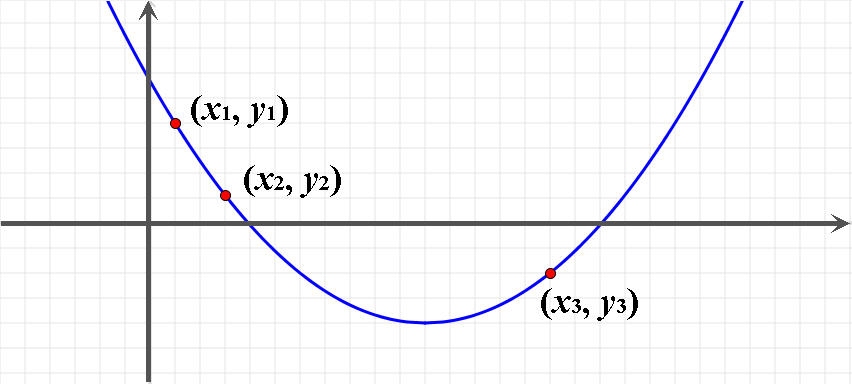
\includegraphics[width=0.45\linewidth]{img/parabool.jpg}
    \end{center}
    
 
    
     \begin{align*}
     &a=\frac{x_3(y_2-y_1)+x_2(y_1-y_3)+x_1(y_3-y_2)}{n} \\ &b=\frac{x_3^2(y_2-y_1)+x_2^2(y_1-y_3)+x_1^2(y_3-y_2)}{-n} \\
     &c=\frac{x_2x_3(x_2-x_3)y_1+x_3x_1(x_3-x_1)y_2+x_1x_2(x_1-x_2)y_3}{n}\\
     &\textrm{met } n= (x_1-x_2)(x_1-x_3)(x_2-x_3)
     \end{align*}
    
     
     In het volgende (onvolledige) Pythonprogramma automatiseren we de berekening van het voorschrift van de parabool en tekenen we meteen ook een parboolsegment over het interval [$x_1$, $x_3$]. \\
     \medskip
     
     \begin{kader}{Python}{Bereken en tekenen van een paraboolsegment door drie gegeven punten}
    1. \qquad import matplotlib as plt\\
    2. \qquad numpy as np\\
    3. \qquad \\
    4. \qquad def parabool(x1, y1, x2, y2, x3, y3):\\
    5. \qquad \qquad \textcolor{red}{noemer= ............}\\
    6. \qquad \qquad \textcolor{red}{a= ............}\\
    7. \qquad \qquad \textcolor{red}{b= ............}\\
    8. \qquad \qquad \textcolor{red}{c= ............}\\
    9. \qquad \qquad x=np.linspace(x1, x3, 100)\\
    10. \qquad \quad \, y=a*x**2+b*x+c\\
    11. \qquad \quad \, plt.plot(x, y, linewidth=2, color='red')\\
    12. \qquad \\
    13. \quad \, print(parabool(-1,2,4,3,14,-1))\\
    14. \quad \, plt.show()\\
    \end{kader}
    
    In lijn 1 en lijn 2 worden externe bibliotheekprogramma's geïmporteerd. Matplotlib, afgekort tot plt, wordt gebruikt om grafieken te plotten. En Numpy, afgekort tot np, wordt gebruikt om het interval [$x_1$,$x_3$] op een handige manier in gelijke segmentjes te verdelen.
    
    \begin{vraagenantwoord}
        \vraag{Vul de definitie van de parabool aan met vier formules. Verklaar daarna de drie laatste regels van deze definitie.}
        \antwoord{In regel $9$ wordt het interval $[x_1,x_3]$ op de $x$-as in $100$ gelijke deelintervalletjes verdeeld. Van deze deelpunten wordt de beeldwaarde berekend met de formule uit regel $10$. Via regel $11$ wordt een plot voorbereid waarbij $101$ puntjes in het vlak met korte lijnstukjes verbonden worden. De lijndikte van deze lijnstukjes is $2$ en de lijnkleur is rood.}
        \vraag{Test het programma uit door het tekenen van een parabool die start in het punt ($-1$, 2) en over het punt (4, 3) verderloopt tot in het punt (14,$-1$).} 
        \vraag{Maak daarna gebruik van dit programma om de figuur hieronder na te tekenen. Voor je hieraan begint teken je de lachende mond over op een ruitjesblad en verzin je coördinaten bij drie punten van elke parabool.}
    \end{vraagenantwoord}
     
   
    \afbeelding[10 cm]{img/mond.jpg}{}{}
  
     
    \end{lesactiviteit}

\begin{multicols}{2}

\section{Theoretisch kader: Wat is het doel van ICT in het wiskundeonderwijs?}
Als afsluiter van deze loep is het goed om na te denken welke rol ICT in het wiskundeonderwijs hoort te spelen. Een bekend model hiervoor is het SAMR-model (Puentedura, 2006) dat je vindt in \autoref{samr}. Het SAMR-model deelt ICT-integratie in twee categorieën in: \textit{verbetering} en \textit{transformatie}. Elke categorie wordt nog verder onderverdeeld in twee niveaus. 

 \afbeelding [6 cm] {img/samr.pdf}{Het SAMR-model van Ruben Puentedure (2006)}{samr}	
 
Het SAMR-model modelleert op die manier het hele spectrum van ICT-integratiemogelijkheden: gaande van technologie als simpele vervanger van bestaande praktijken, tot technologie als ontstaansreden van nieuwe praktijken, die zonder technologie gewoon onmogelijk zouden zijn. In de vorige paragrafen maakten we alle niveaus concreter. De kritische lezer zal misschien opmerken dat het model ICT-integratie altijd als een positieve evolutie ziet, terwijl het ook een verslechtering kan zijn (bv. een krijtbord vervangen door een smartboard, dat zowel qua gebruiksgemak als grootte vaak niet kan tippen aan het gewone krijtbord.


\subsection*{(S) Vervanging}
Op dit niveau is technologie louter de vervanger van bestaande praktijken, zonder dat er functioneel enige verbetering mee gemoeid gaat. Denk aan een leraar die een oefening op een smartboard noteert in plaats van op een krijtbord, een leraar die zijn cursus in pdf naar de leerlingen mailt in plaats van ze afdrukt, of aan een handgeschreven taak die niet meer tijdens de les wordt afgegeven. In plaats daarvan  trekt de leerling foto’s van zijn papieren, maakt er één pdfje van en uploadt de taak via de uploadzone van Smartschool. De leraar geeft vervolgens zijn feedback digitaal. Wanneer we in maart 2020 allemaal verplicht aan het werk moesten met afstandsonderwijs, waren we in eerste instantie op dit niveau aan het nadenken over onze aanpak: hoe kunnen we online voor elkaar krijgen wat we altijd al deden in het vertrouwde klaslokaal?

\subsection*{(A) Versterking}
Op dit niveau vervangt technologie bestaande praktijken, maar voegt er ook enkele functionele verbeteringen aan toe. Denk aan het digitaal afnemen van een multiple-choicetoets met enkele wiskundige inzichtsvragen, die automatisch verbeterd kan worden en waarbij een leerling meteen feedback krijgt op gemaakte fouten. Dat heeft een papieren multiple-choicetoets niet te bieden. In één van de inleidende lessen over goniometrische functies, projecteert de leraar de grafiek van $f(x)=\sin x$ om de kenmerken van de sinusfunctie klassikaal te onderzoeken. De leraar kan zo in- en uitzoomen en navigeren naar interessante delen van de grafiek. Wanneer de leraar de sinusfunctie op bord zou tekenen, zou nog steeds hetzelfde leerdoel centraal staan (namelijk het onderzoeken van de functiekenmerken van $f(x)=\sin x$), maar zouden die functionele verbeteringen van in- en uitzoomen ontbreken. Het voorbeeld van de normaalverdeling met GeoGebra en de visualisatie van extremumproblemen vallen ook onder deze rubriek, net als het voorbeeld van de families krommen (paragraaf 4.3).

\subsection*{(M) Verandering}
Verandering is het eerste niveau waarbij technologie bestaande praktijken gaat transformeren. Op dit niveau stelt technologie ons in staat om een taak fundamenteel te herdenken, waardoor het leerdoel dat centraal staat mee verandert. Denk hierbij aan alle nieuwe oplossingsstrategieën die de invoering van het grafisch rekentoestel met zich meebracht. In plaats van een langgerekt functieonderzoek tot en met de tweede afgeleide met een schets van de grafiek van de functie als eindpunt, lag het ineens binnen handbereik van elke leerling om de functie van meet af aan te plotten. Dat maakte allerlei nieuwe leerdoelen mogelijk: het grafisch opstellen van tekentabellen, het grafisch oplossen van extremumvraagstukken bij een inleidend hoofdstuk over veeltermfuncties, het oplossen van vergelijkingen door het plotten van de overeenkomstige grafieken... Ook het onderwijzen van meetkunde ziet er door de opkomst van technologie toch flink anders uit. Waar een leraar vroeger aan het bord zich vaak tot één tekening beperkte om een voorbeeld van een stelling te geven en die vervolgens te bewijzen, kunnen leerlingen nu via applets enkele punten verslepen, om zo `experimenteel' de stelling na te gaan op tientallen voorbeelden. Indien er voorwaarden gekoppeld worden aan de stelling (bv. enkel van toepassing op rechthoekige driehoeken), kunnen ze die vaak zelf ontdekken.

\subsection*{(R) Herdefiniëring}
Herdefiniëring behelst alle taken die zonder technologie gewoon ondenkbaar zouden zijn. Denk bv. aan leerlingen die tijdens de lessen statistiek grote, realistische datasets analyseren, wat ondenkbaar is zonder de inzet van ICT. Het gebruik van een computeralgebraysteem (CAS) laat toe om bv. realistische modelleeropdachten in het kader van integraalrekening aan te gaan. Eenvoudige functies met getallen die `mooi uitkomen' blijven nodig om tot de kern van de zaak te komen. Maar daarna kun je complexere gevallen onderzoeken die minder goed uitkomen maar waar de computer het rekenwerk overneemt. De focus ligt dan niet op het uitrekenen maar op de analyse, zoals bij het voorbeeld van de telecomoorlog (paragraaf 4.2). 

\subsection*{Tot slot}
Het SAMR-model geeft geen waardeoordeel over de verschillende niveaus van ICT-integratie. Het zijn geen fases die je in een bepaalde volgorde moet doorlopen en die altijd moeten uitmonden in \textit{herdefiniëring}. Het biedt wel een kader om de stand van zaken in kaart te brengen en na te denken over hoe je jouw wiskunde-onderwijs kunt verbeteren door het doeltreffend inzetten van ICT. De twee niveaus onder verbetering worden doorgaans geassocieerd met meer leraargestuurde instructie, de twee transformatieniveaus laten leerlingen vaak zelf oplossingen exploreren, en zijn daarom doorgaans geassocieerd met meer leerlinggerichte werkvormen. Als de dag des oordeels zich aandient en de grafische rekenmachine op school definitief de baan ruimt voor een laptop, is het goed om als vakgroep voorbereid te zijn. Het is nu de moment om deze verandering voor te bereiden en na te denken wat de kansen en mogelijkheden zijn van nieuwe technologie, wat je ermee kunt en wilt bereiken. Als het doel duidelijk is, is er meer motivatie om de praktische bezwaren die eigen zijn aan elke verandering, aan te pakken.


	\section{Hoe zit het in het hoger onderwijs en in Nederland?}
	Het hoger onderwijs heeft veelal de stap met de grafische rekenmachine overgeslagen. Studenten moeten soms een eenvoudige rekenmachine kopen voor bepaalde examens omdat ze geen grafisch toestel mogen gebruiken. Een rondvraag bij verschillende faculteiten levert een uiterst divers beeld op. Aan de universiteit wordt meestal niet met een grafische rekenmachine gewerkt (al zijn er uitzonderingen). Soms wordt nog alle ICT geweerd, maar meer en meer wordt bij vakken waarbij dat aangewezen is, gewerkt met wiskundige software op de computer. Niet het toestel telt, wel het feit dat ICT-tools een plaats hebben in het huidige wiskundeonderwijs. Het kan dan gaan over software die numerieke berekeningen maakt of over computeralgebrasoftware. Vaak wordt dan via een aparte taak getoetst of studenten dat onder de knie hebben en komt de software dan niet meer aan bod op het examen. 
	 
In Nederland zijn er al langer centrale examens. Welke rekenmachines, software mag daar gebruikt worden? Voor elk niveau staat er zorgvuldig beschreven wat kan en niet kan. Op de website van de centrale examens vind je de lijst van toegestane hulpmiddelen voor vmbo en voor vwo/havo. Deze lijsten worden elk jaar aangepast. De regels gelden alleen voor het centrale examen. Scholen mogen van deze regels afwijken als het gaat om een schoolexamen, eigen toetsen... De lijst geeft aan wat een eenvoudige rekenmachine moet kunnen en ook niet mag kunnen, hoeveel tekstregels een wetenschappelijke rekenmachine mag hebben, welke types grafische rekenmachines er gebruikt mogen worden. Die laatste moeten verplicht in examenstand gezet worden.

Als het bij ons ook tot centrale examens komt, is er alvast daarvoor ook nog veel nood aan afspraken hieromtrent!

Dankjewel Bart Janssens, Tom Deckers,  Mathias Stichelbaut, Michel Roelens en Stijn Meuwissen voor jullie inbreng!
%	\begin{kader}{Kadertype}{Titel van dit kader}
%		\lipsum[1][1-2]
%	\end{kader}

\end{multicols}	


%% LESACTIVITEIT %%%%%%%%%%%%%%%%%%%%%%%%%%%%%%%%%%%%%%%%%%%%%%%%%%%%%%%%%%%%%%%
%% Gebruik de {lesactiviteit} omgeving om een lesactiviteit aan te geven. Gebruik dit enkel BUITEN een multicols omgeving!
%\begin{lesactiviteit}{Titel van de lesactiviteit}
	
%	\begin{vraagenantwoord}
%		\vraag{\lipsum*[1][1-2]}
%	\antwoord{\lipsum*[1][3-4]}
		
%		\vraag{\lipsum*[1][1-2]}
%		\antwoord{\lipsum*[1][3-4]}
%	\end{vraagenantwoord}
	
%\end{lesactiviteit}


\stopcontents[inhoudloep]		% om inhoud voor het loep artikel te eindigen


%% BRONNEN %%%%%%%%%%%%%%%%%%%%%%%%%%%%%%%%%%%%%%%%%%%%%%%%%%%%%%%%%%%%%%%%%%%%%
\begin{bronnen}

\item Conradi, R. (2016, 1 september). Het SAMR-model: zo integreert u onderwijstechnologie. \emph{Onderwijs van Morgen.}
\url{https://www.onderwijsvanmorgen.nl/samr-model-zo-integreert-u-onderwijstechnologie}

\item Drehling, W., Merkert, P. en van Kruysbergen, N. (2022, 5 mei). Python voor iedereen. \emph{C'T, IT-magazine voor de liefhebber}, 86-100. F\&L Media BV. ISSN 1388-0276

\item Puentedura, R.R. (2006).\textit{ Transformation, technology, and education}. http://hippasus.com/resources/tte/

\item Statistics \& Data. \emph{The Most Popular Programming Languages – 1965/2021.}\\
\url{https://statisticsanddata.org/data/the-most-popular-programming-languages-1965-2021/}
\item \url{https://www.kennisnet.nl/app/uploads/kennisnet/publicatie/Schoolbeleid_voor_smartphones.pdf} 
\item \url{https://www.leraar24.nl/2613136/hoe-ga-je-slim-om-met-smartphones-in-de-klas/ } 
\item \url{https://www.geogebra.org/m/KtZZJ8SR} Examenmodus GeoGebra 
\item \url{https://www.examenblad.nl/onderwerp/hulpmiddelen-centrale-examens/2022?topparent=vg41h1h4i9qe}
\item \url{https://www.geogebra.org/m/ysdsbbrx} Telecomoorlog.
\item \url{https://www.geogebra.org/classic/D7GBC0x9} Convergerende rij.
\item \url{https://www.geogebra.org/m/cwbunwjn} Meetkunde met Geogebra.


\end{bronnen}